\documentclass{article}\usepackage{graphicx, color}
%% maxwidth is the original width if it is less than linewidth
%% otherwise use linewidth (to make sure the graphics do not exceed the margin)
\makeatletter
\def\maxwidth{ %
  \ifdim\Gin@nat@width>\linewidth
    \linewidth
  \else
    \Gin@nat@width
  \fi
}
\makeatother

\IfFileExists{upquote.sty}{\usepackage{upquote}}{}
\definecolor{fgcolor}{rgb}{0.2, 0.2, 0.2}
\newcommand{\hlnumber}[1]{\textcolor[rgb]{0,0,0}{#1}}%
\newcommand{\hlfunctioncall}[1]{\textcolor[rgb]{0.501960784313725,0,0.329411764705882}{\textbf{#1}}}%
\newcommand{\hlstring}[1]{\textcolor[rgb]{0.6,0.6,1}{#1}}%
\newcommand{\hlkeyword}[1]{\textcolor[rgb]{0,0,0}{\textbf{#1}}}%
\newcommand{\hlargument}[1]{\textcolor[rgb]{0.690196078431373,0.250980392156863,0.0196078431372549}{#1}}%
\newcommand{\hlcomment}[1]{\textcolor[rgb]{0.180392156862745,0.6,0.341176470588235}{#1}}%
\newcommand{\hlroxygencomment}[1]{\textcolor[rgb]{0.43921568627451,0.47843137254902,0.701960784313725}{#1}}%
\newcommand{\hlformalargs}[1]{\textcolor[rgb]{0.690196078431373,0.250980392156863,0.0196078431372549}{#1}}%
\newcommand{\hleqformalargs}[1]{\textcolor[rgb]{0.690196078431373,0.250980392156863,0.0196078431372549}{#1}}%
\newcommand{\hlassignement}[1]{\textcolor[rgb]{0,0,0}{\textbf{#1}}}%
\newcommand{\hlpackage}[1]{\textcolor[rgb]{0.588235294117647,0.709803921568627,0.145098039215686}{#1}}%
\newcommand{\hlslot}[1]{\textit{#1}}%
\newcommand{\hlsymbol}[1]{\textcolor[rgb]{0,0,0}{#1}}%
\newcommand{\hlprompt}[1]{\textcolor[rgb]{0.2,0.2,0.2}{#1}}%

\usepackage{framed}
\makeatletter
\newenvironment{kframe}{%
 \def\at@end@of@kframe{}%
 \ifinner\ifhmode%
  \def\at@end@of@kframe{\end{minipage}}%
  \begin{minipage}{\columnwidth}%
 \fi\fi%
 \def\FrameCommand##1{\hskip\@totalleftmargin \hskip-\fboxsep
 \colorbox{shadecolor}{##1}\hskip-\fboxsep
     % There is no \\@totalrightmargin, so:
     \hskip-\linewidth \hskip-\@totalleftmargin \hskip\columnwidth}%
 \MakeFramed {\advance\hsize-\width
   \@totalleftmargin\z@ \linewidth\hsize
   \@setminipage}}%
 {\par\unskip\endMakeFramed%
 \at@end@of@kframe}
\makeatother

\definecolor{shadecolor}{rgb}{.97, .97, .97}
\definecolor{messagecolor}{rgb}{0, 0, 0}
\definecolor{warningcolor}{rgb}{1, 0, 1}
\definecolor{errorcolor}{rgb}{1, 0, 0}
\newenvironment{knitrout}{}{} % an empty environment to be redefined in TeX

\usepackage{alltt}
%\VignettePackage{rlandscape}
%\VignetteDepends{rlandscape}
%\VignetteIndexEntry{rlandscape tutorial}
\usepackage[margin=1.0in]{geometry}
\author{Gregor Passolt}
\title{Generating landscapes with the \code{rlandsacpe} package}
\date{\today}
\newcommand{\code}[1]{{\tt #1}}

\begin{document}

\maketitle
\tableofcontents

The \code{rlandscape} package is intended to make it easy to simulate random landscapes
for testing harvest scheduling models.
This vignette will cover use of the two primary functions,
\code{rlandscape} and \code{rland}, and is aimed at users that are new to R.
Most users will probably find \code{rland} the more useful,
but should have a basic understanding of what \code{rlandscape} does so they know what they're getting.
To learn about how \code{rlandcsape} works, please refer to
Gregor Passolt, Miranda J. Fix, and Sandor F. Toth (in review).
A Voronoi Tessellation-based Approach to Generate Hypothetical Forest Landscapes,
Canadian Journal of Forest Research.

\section{Generating a single landscape with \code{rlandscape}}

The foundation of the package is \code{rlandscape}, which generates a single landscape at a time.
Its output (a landscape object) can be assigned to a variable for analysis or saving.
The first step is to download the \code{rlandscape} package.
If you're reading this vignette, that's probably already done, but just in case the command is
\verb|install.packages("rlandscape")|.
Other dependencies will be installed automatically, which may take a minute.
This only needs to be performed once.
Every time you start a new R session, you will need to load the package, which can be done
either with the \verb|require| or \verb|library| commands.

\begin{knitrout}
\definecolor{shadecolor}{rgb}{0.969, 0.969, 0.969}\color{fgcolor}\begin{kframe}
\begin{alltt}
\hlfunctioncall{library}(rlandscape)  \hlcomment{## loading the package}
\end{alltt}
\end{kframe}
\end{knitrout}


Now that the package is loaded, all the associated functions are available.
Let's get started creating a landscape

\begin{knitrout}
\definecolor{shadecolor}{rgb}{0.969, 0.969, 0.969}\color{fgcolor}\begin{kframe}
\begin{alltt}
myLand <- \hlfunctioncall{rlandscape}()
\hlfunctioncall{plot}(myLand)
\end{alltt}
\end{kframe}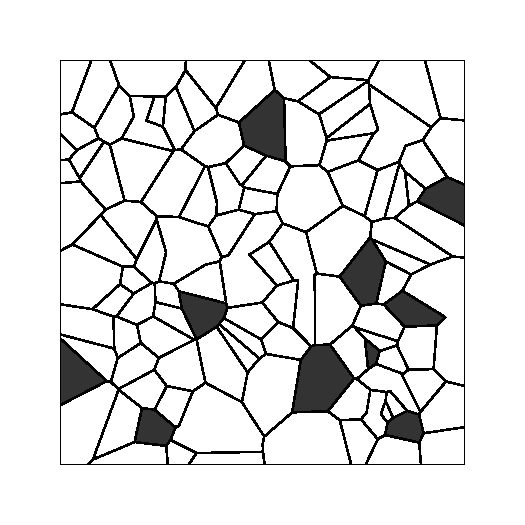
\includegraphics[width=\maxwidth]{figure/rlandscape1} \begin{kframe}\begin{alltt}
myLand$stats
\end{alltt}
\begin{verbatim}
##   nOut degMean degSD areaCV hAsp  n1 n2 n3 n4 pMerge pHole
## 1  100    4.86 1.511  55.15    1 100  0  0  0    0.1   0.1
\end{verbatim}
\end{kframe}
\end{knitrout}


Particular features of this landscape can be extracted using the \verb|$| operator.
The \code{stats} display the final number of
polygons (nOut), the mean of the degree distribution (degMean),
the standard deviation of the degree distribution (degSD),
the coefficient of variation of the area distribution (areaCV),
the horizontal:vertical aspect ratio (hAsp),
the number of points placed by each of the 4 point placement methods (uniform, lattice, cluster,
inhibition, respectively),
the proportion of edges deleted to merge two polygons together (pMerge),
and the proportion of polygons deleted to become holes (pHole).
The adjacency table is available as \code{adj}, and the areas are in the \code{dir.area} column
of a summary table that includes information for all of original points, such as their x-y
coordinates, whether they were deleted, and whether they were merged with another polygon.
Note that, due to the deletions and merge events, the polygon numbering will not be sequential.
For example, if polygon 2 is deleted, another polygon will not be renamed ``2''.

\begin{knitrout}
\definecolor{shadecolor}{rgb}{0.969, 0.969, 0.969}\color{fgcolor}\begin{kframe}
\begin{alltt}
\hlfunctioncall{head}(myLand$adj)
\end{alltt}
\begin{verbatim}
## [[1]]
## [1]  13  20  67 103
## 
## [[2]]
## [1]  16  32  39  42  62  69 101
## 
## [[3]]
## [1]  51  89 103 115
## 
## [[4]]
## [1] 21 30 46 49 83
## 
## [[5]]
## [1]  6 15 49 83
## 
## [[6]]
## [1]  5 15 23
\end{verbatim}
\begin{alltt}
\hlfunctioncall{head}(myLand$summary)
\end{alltt}
\begin{verbatim}
##           x      y n.tri del.area  del.wts n.tside nbpt dir.area  dir.wts
## [1,] 0.6262 0.9559     6 0.008947 0.010097       5    2 0.010539 0.010539
## [2,] 0.2227 0.9439     9 0.008992 0.010147       7    2 0.013722 0.013722
## [3,] 0.7180 0.8291     5 0.004188 0.004727       5    0 0.005055 0.005055
## [4,] 0.5592 0.3903     6 0.005205 0.005874       6    0 0.006399 0.006399
## [5,] 0.4710 0.2936     5 0.003600 0.004062       5    0 0.003873 0.003873
## [6,] 0.4586 0.2792     4 0.002910 0.003285       4    0 0.003542 0.003542
##      holeThese mergedWith
## [1,]         0          0
## [2,]         0          0
## [3,]         0          0
## [4,]         0          0
## [5,]         0          0
## [6,]         0          0
\end{verbatim}
\end{kframe}
\end{knitrout}



You can give arguments to \code{rlandcsape} to alter the landscape under construction.
For example, a landscape of 500 polygons, with a 2:1 aspect ratio and a very patchy composition
would be given by:

\begin{knitrout}
\definecolor{shadecolor}{rgb}{0.969, 0.969, 0.969}\color{fgcolor}\begin{kframe}
\begin{alltt}
land2 <- \hlfunctioncall{rlandscape}(n = 500, hAsp = 2, pHole = 0.5)
\end{alltt}
\end{kframe}
\end{knitrout}


You can access the helpfile for \code{rlandscape} by entering \code{?rlandscape} at the console.
It describes all of the options available as well as the defaults.



\section{Batch generation using \code{rland}}

The \code{rland} function is used when, rather than specifying control parameters for the
point processes used to generate landscapes, you want to specify the characteristics of the
resulting landscape. It also makes it easy to generate and save any number of landscapes.

The most workhorse arguments to \code{rland} are \code{targets} and \code{bounds}.
The \code{targets} sets the range of landscape characteristics the algorithm will ``aim'' for, while
\code{bounds} sets the range of landscape characteristics that will be accepted.
The target ranges must fall inside the bounds ranges.
See the \code{rland} help file (enter \code{?rland}) for information on defaults.

\code{Rland} is designed to write its output to files rather than display it in R. 
When you start an R session, there is a ``working directory'' to which, by default, R will save
files (or look for files to load).
You can see or change the current working directory with the commands
\code{getwd} and \code{setwd}, or through file menus which depend on your operating system
and interface.
The working directory is where \code{rland} will write its output unless you specify a full filepath.
The \code{filename} argument to \code{rland} is for the name of the run.
For example, if you use \verb|filename = "land-sim"|
and create 10 landscapes, they will be named
and saved as \code{land-sim-01} to \code{land-sim-10} in the working directory.
To have them saved somewhere else, you could set
\verb|filename = "C:/otherDirectory/land-sim"|.
The default filename is \code{"landscape"}.

\subsection{Examples}
So, if you wanted to generate 50 landscapes with between 200 and 300 polygons, 
and save the plots of each landscape, this would do it:

\begin{verbatim}
    rland(targets = list(n = c(200, 300)),
          bounds = list(n = c(200, 300)),
          reps = 50,
          filename = "run1",
          savePlot = TRUE)
\end{verbatim}

A similar run with more specifications would look like this:
\begin{verbatim}
    rland(targets = list(n = c(200, 300),
                         degMean = c(4.8, 5.2),
                         areaCV = c(50, 70),
                         hAsp = c(1, 5)),
          bounds = list(n = c(175, 325),
                        degMean = c(4.8, 5.2),
                        areaCV = c(45, 75)),
          reps = 50, filename = "run2", savePlot = TRUE)
\end{verbatim}

By default, the plots are not saved, but the adjacencies and areas are, as well as a summary
table giving descriptive statistics about each of the landscapes. This can be viewed in R
by

\begin{verbatim}
    run1.summary <- read.table("run1_summary.csv")
    head(run1.summary)
    hist(run1.summary$degMean) ## plotting a histogram of the degree means
\end{verbatim}

A assortment of 100 landscapes with random characteristics is created by
\begin{verbatim}
   rland(reps = 100, method = "random", filename = "random_landscape")
\end{verbatim}

\subsection{GUI}

A graphical user interface (GUI) is available to interact with \code{rland}.
All the arguments of \code{rland} can be accessed through the GUI.
To start the GUI, simply enter \code{rland.gui()} in the R console.

\end{document}
